\section{System and Method}
\label{sec:system}

The question of when federation helps needs a classifier cheap enough to run on every request at a gateway and small enough that exchanging it costs next to nothing. The system built to test this has two roles. An \emph{edge gateway} scores HTTP requests locally with a linear model and never transmits payloads. A \emph{cloud aggregator} accepts MAC-tagged parameter updates from enrolled gateways, combines them, and returns a global model. Figure~\ref{fig:architecture} shows the flow. The gateway is a web application firewall (WAF) enforcement point. It can sit inside a zero-trust deployment, where it supplies one per-request check on payload content, but it does not establish requester identity or device posture and is not itself a zero-trust architecture. Trust assumptions, adversaries and the limits of each control are stated once, in Section~\ref{sec:sec-threat}; this section describes mechanisms only.

\begin{figure}[t]
\centering
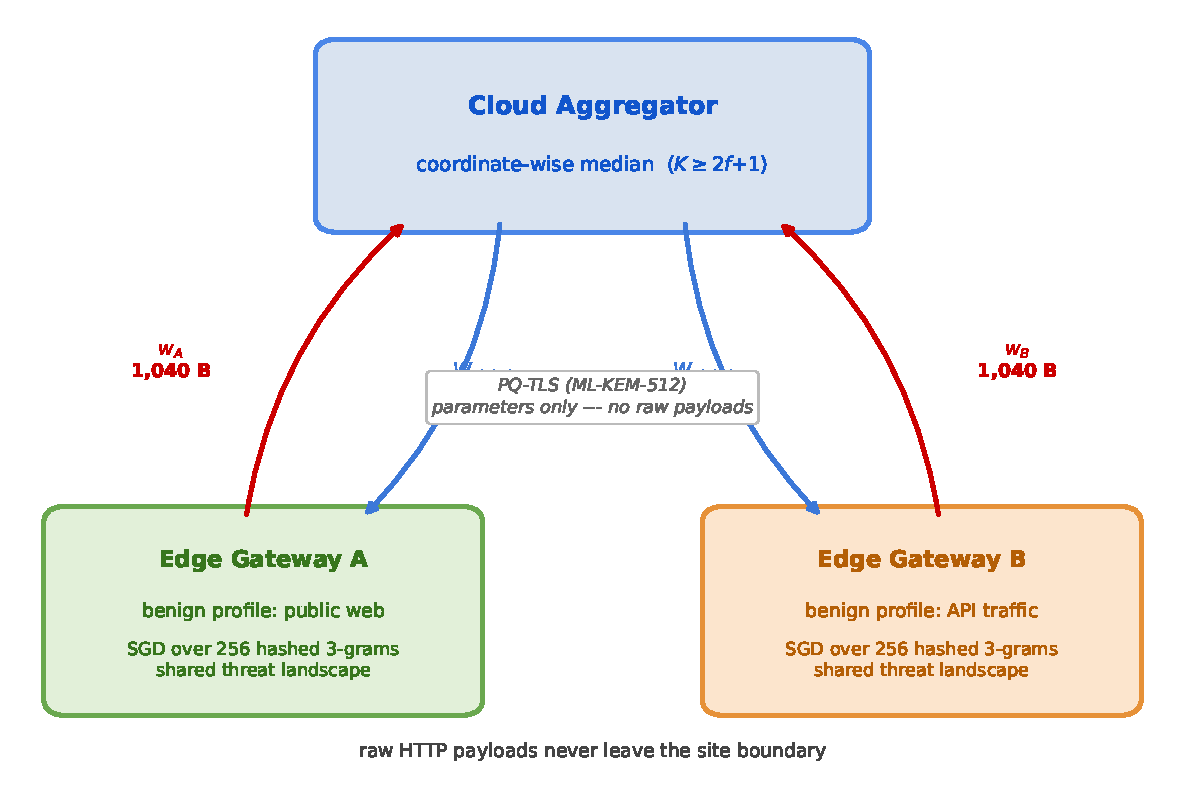
\includegraphics[width=\linewidth]{figures/fl_architecture.pdf}
\caption{System architecture. Edge gateways score requests locally and upload MAC-tagged weight vectors over plain HTTP; the cloud aggregator authenticates, gates and aggregates them. Raw traffic stays at the edge.}
\label{fig:architecture}
\end{figure}

\subsection{Features and Classifier}
\label{sec:sys-features}
Feature computation lives in one module, \texttt{fedzta\_features.py}, imported by the gateway, the aggregator and the profiler so that every party buckets n-grams identically. The unit that is featurised is a \emph{context} $P$: one string such as a path, a query string, a header value or a body. Each context maps to $\mathbf{x}(P)\in\mathbb{R}^{D+3}$ with $D=256$, i.e.\ $259$ dimensions:
\begin{equation}
\mathbf{x}(P) = \big[\, \hat{\mathbf{h}}(P) \;\big|\; \tfrac{|P|}{100} \;\big|\; \tfrac{s(P)}{20} \;\big|\; \tfrac{H(P)}{5} \,\big].
\end{equation}
Here $\hat{\mathbf{h}}(P)$ is the $\ell_2$-normalised histogram of lower-cased character trigrams hashed into $D$ buckets by a polynomial rolling hash (multiplier $131$, $32$-bit state), $s(P)$ counts non-alphanumeric characters, and $H(P)$ is the Shannon entropy of the character distribution. The polynomial hash replaced MD5 for speed on the Cortex-A72 (0.242\,ms versus 0.404\,ms per request in an earlier profiling run). The scaling constants $(100,20,5)$ are fixed a priori, so no scaler is shipped to the edge and no test statistics reach training.

The classifier is logistic regression, $p(\mathbf{x})=\sigma(\mathbf{w}^\top\mathbf{x}+b)$, with the logit clipped to $[-250,250]$. The model has $259$ coefficients and an intercept, $1{,}040$ bytes in single precision, which is also the size of one synchronisation payload.

\subsection{Training Unit and Scoring Unit}
\label{sec:sys-units}
Training and inference operate on different units. In training, each sampled string, benign or malicious, is wrapped in one of seven synthetic request contexts (Section~\ref{sec:eval-setup}) and the \emph{wrapped string as a whole} is one example, featurised as a single context $P$. No example is a full multi-field request. At inference the gateway builds a list $\mathcal{C}(r)$ of contexts from the request, scores each separately with the same model, and takes the maximum (Section~\ref{sec:sys-waf}). The scoring rule therefore assumes that the field carrying an attack looks, to the model, like one of the wrapped training strings. That assumption is untested on captured traffic. Taking the maximum over several fields also raises the false-positive rate relative to scoring one field, because every extra benign context is another chance to cross the threshold.

\subsection{Offline Training and Online Aggregation}
\label{sec:sys-agg}
Two aggregation procedures appear in this paper and they are not interchangeable. \emph{Offline federated averaging} produced the shipped model and all accuracy results; \emph{online coordinate-wise median} runs in the deployed aggregator and is the subject of the poisoning study.

\paragraph{Offline FedAvg.}
Training follows federated averaging~\cite{mcmahan2017} over two simulated gateways (\texttt{fl\_simulation\_v4.py}, \texttt{train\_production\_model.py}). Each node holds an \texttt{SGDClassifier} with logistic loss, $\ell_2$ penalty $\alpha=10^{-4}$ and constant learning rate $\eta_0=0.01$. In each of $R=20$ rounds every node starts from the global parameters, trains for $E=30$ local epochs on its own data, and the server forms the sample-weighted average
\begin{equation}
\theta^{(t+1)} = \sum_k \tfrac{n_k}{n}\,\theta_k^{(t)}, \qquad n=\sum_k n_k .
\end{equation}
Train and test sets are disjoint at the level of unique payloads. The two nodes differ by benign profile (public web versus API), the configuration chosen from the controlled matrix of Section~\ref{sec:eval-matrix} because it was the only cell in which federation exceeded both silos, a selection made on test results.

\paragraph{Online median.}
The deployed aggregator (\texttt{robust\_cloud.py}) keeps the latest update of each enrolled client and recomputes the global model on every accepted update (Algorithm~\ref{alg:aggregator}). With $K$ stored updates the default rule is the coordinate-wise median~\cite{yin2018},
\begin{equation}
w_j = \operatorname{median}\{w_{k,j}\}_{k=1}^{K}, \qquad b = \operatorname{median}\{b_k\}_{k=1}^{K},
\end{equation}
with a trimmed mean or plain mean selectable for comparison. The median tolerates $f$ Byzantine clients only while $K\ge 2f+1$. The \texttt{/weights} endpoint reports $f_{\max}=\max(0,\lfloor (K-1)/2\rfloor)$ and a \texttt{robust} flag, so a deployment with $K<3$ is visibly unprotected. Gateways keep training locally between syncs only through the anchor replay of Section~\ref{sec:sys-waf}; the offline FedAvg schedule is not run online.

Each update must pass, in order, authentication (Section~\ref{sec:sys-auth}), a per-client rate limit (default one update per $5$\,s), dimension and finiteness checks, and a \emph{norm gate}. The gate rejects an update whose $\ell_2$ norm, relative to a reference norm, falls outside $[1/\rho,\rho]$ with $\rho=4$. The reference is the median norm of the other peers when at least two have reported; with exactly one other peer, the larger of that peer's norm and the bootstrap model's norm; otherwise the bootstrap norm. The gate therefore stays active at $K=2$. Section~\ref{sec:sec-poison} discusses what it does and does not stop.

\subsection{Authenticated Updates}
\label{sec:sys-auth}
\texttt{fedzta\_auth.py} binds each update to an enrolled gateway. Enrolment (\texttt{enroll\_peer.py}) issues a 256-bit secret from the OS CSPRNG. An update is the body $\{\text{client\_id},\mathbf{w},b,n,\text{ts},\text{nonce}\}$, serialised canonically (sorted keys, fixed separators) and tagged with HMAC-SHA256~\cite{rfc2104}; we call the result a MAC-tagged update. Verification checks that the client is enrolled (unknown and malformed identifiers receive the same response), that the tag matches under a constant-time comparison, that the timestamp lies within $\pm120$\,s, and that the nonce has not appeared in the last $300$\,s (\texttt{ReplayGuard}). A symmetric MAC needs only \texttt{hmac} and \texttt{hashlib} from the Python standard library, which keeps the edge dependency-free. Symmetric keys give authenticity and freshness but not non-repudiation (Section~\ref{sec:sec-limits}).

\subsection{Transport and the ML-KEM Benchmark}
\label{sec:sys-pqc}
The live transport is plain HTTP carrying HMAC-authenticated JSON: \texttt{/update} and \texttt{/weights} are neither encrypted nor protected by TLS. ML-KEM-512~\cite{fips203} exists in the repository as a standalone key-exchange benchmark (\texttt{cloud\_pqc.py}, \texttt{edge\_pqc.py}): the aggregator serves a public key at \texttt{/pubkey}, the gateway encapsulates against it, posts the ciphertext to \texttt{/exchange}, and both sides derive the same shared secret. That secret is not used to encrypt any update. The system provides authentication of the update path and no confidentiality against a network observer; this paper makes no post-quantum security claim.

\subsection{Gateway}
\label{sec:sys-waf}
The gateway (\texttt{continuous\_waf.py}, Algorithm~\ref{alg:gateway}) is a multi-threaded HTTP server. For each GET, POST or PUT request it builds $\mathcal{C}(r)$: the URL path, the percent-decoded query string, the \texttt{User-Agent}, \texttt{Referer} and \texttt{Cookie} header values, and for POST and PUT the body truncated to $8$\,KB. The request score is the maximum context score,
\begin{equation}
s(r) = \max_{P\in\mathcal{C}(r)} p\big(\mathbf{x}(P)\big),
\end{equation}
so a payload in one field is not diluted by benign neighbours, and the request is blocked with HTTP~403 when $s(r)\ge\tau$. In \emph{shadow mode} the gateway counts would-be blocks but forwards everything; the \emph{failure policy} selects fail-open (the default, forwarding on internal error) or fail-closed. Sockets time out after $5$\,s, non-numeric \texttt{Content-Length} values are rejected, and bodies are read only up to the cap. Counters are updated under a lock, and \texttt{/health} and \texttt{/metrics} expose liveness and block counts.

\paragraph{Decision threshold.}
The offline profiler uses $\tau=0.5$; the deployed gateway uses $\tau=0.15$. The shipped model was trained on augmented benign data (JSON and form bodies, varied lengths, prose), which moves the intercept to $b\approx-5.57$ and lowers attack probabilities, and $\tau$ was lowered to compensate. Held-out behaviour at this threshold is reported in Section~\ref{sec:evaluation}, not here.

\paragraph{Anchor replay.}
An earlier gateway trained on its own confident predictions, which lets the model reinforce its own errors; that loop was removed. Local adaptation is now a replay of a small operator-verified list of labelled payloads (\texttt{anchor\_set.json}) through one SGD step each ($\eta=0.05$) every $60$\,s. The anchor set limits drift and offers a hook for verified labels; new knowledge is supposed to arrive through federation.

\paragraph{Synchronisation.}
Every $15$\,s the gateway uploads a MAC-tagged snapshot (weights, bias, sample count), downloads the global model, and adopts it if its length is $259$, persisting it atomically (write, \texttt{fsync}, rename). Rejections (401, 409, 429) are logged and the gateway keeps its current model, so an aggregator outage never stops inspection. Each published global model is versioned to permit rollback.

\subsection{Procedures}
\label{sec:sys-alg}
\begin{algorithm}[t]
\caption{Edge gateway: inspection and synchronisation}
\label{alg:gateway}
\begin{algorithmic}[1]
\Require model $(\mathbf{w},b)$, threshold $\tau$, anchor set $\mathcal{A}$, secret $k$, interval $T$
\Procedure{Inspect}{request $r$}
  \State $\mathcal{C}\gets$ path, decoded query, \texttt{User-Agent}, \texttt{Referer}, \texttt{Cookie}, body$[{:}8192]$
  \State $s\gets \max_{P\in\mathcal{C}} \sigma(\mathbf{w}^\top\mathbf{x}(P)+b)$
  \If{$s\ge\tau$ \textbf{and not} shadow mode} \Return 403 \Else{} \Return forward \EndIf
\EndProcedure
\Procedure{SyncLoop}{}
  \While{true} wait $T$ seconds
    \State $m\gets (\textsc{Body}(\text{id},\mathbf{w},b,n,\text{ts},\text{nonce}),\ \textsc{HMAC}_k(\cdot))$; POST $m$ to cloud
    \State $(\mathbf{w}_g,b_g)\gets$ GET global model
    \If{$|\mathbf{w}_g|=259$} $(\mathbf{w},b)\gets(\mathbf{w}_g,b_g)$; persist atomically \EndIf
  \EndWhile
\EndProcedure
\Procedure{AnchorLoop}{}
  \While{true} wait $60$ s
    \ForAll{$(P,y)\in\mathcal{A}$} $\mathbf{w}\gets\mathbf{w}-\eta(\sigma(\mathbf{w}^\top\mathbf{x}(P)+b)-y)\,\mathbf{x}(P)$ (and $b$ likewise) \EndFor
  \EndWhile
\EndProcedure
\end{algorithmic}
\end{algorithm}

\begin{algorithm}[t]
\caption{Cloud aggregator: handling an update}
\label{alg:aggregator}
\begin{algorithmic}[1]
\Require enrolled secrets $\{k_c\}$, replay guard, norm limit $\rho$, rate interval $\delta$
\Procedure{OnUpdate}{message $m$}
  \If{\textbf{not} \textsc{Verify}$(m,\{k_c\})$} \Return 401 \EndIf \Comment{enrolled, HMAC, timestamp, nonce}
  \If{client updated less than $\delta$ ago} \Return 429 \EndIf
  \If{$|\mathbf{w}|\ne 259$ \textbf{or} non-finite} \Return 400 \EndIf
  \State $\text{ref}\gets$ median norm of other peers (or bootstrap norm fallback)
  \If{$\|\mathbf{w}\|_2/\text{ref}\notin[1/\rho,\rho]$} \Return 409 \EndIf
  \State $\text{latest}[c]\gets(\mathbf{w},b)$
  \State $w_j\gets\operatorname{median}_k\, w_{k,j}\ \ \forall j$;\quad $b\gets\operatorname{median}_k b_k$; publish version
  \State \Return 200
\EndProcedure
\end{algorithmic}
\end{algorithm}

\subsection{Implementation Status}
\label{sec:sys-status}
Table~\ref{tab:sys-status} records what the repository implements and what it does not, so that later sections can be read against it. Each row corresponds to a code path; no feature that a row lists as absent or off the live path is assumed anywhere in the evaluation.

\begin{table}[t]
\centering
\caption{Implementation status of the prototype.}
\label{tab:sys-status}
\small
\begin{tabular}{@{}p{2.5cm}p{5.3cm}@{}}
\toprule
\textbf{Area} & \textbf{Status} \\ \midrule
Inspection & GET, POST, PUT; path, query, \texttt{User-Agent}, \texttt{Referer}, \texttt{Cookie}, body ($\le8$\,KB); per-context score, maximum taken \\
Update auth & Enrolment allowlist, HMAC-SHA256, timestamp, single-use nonce (consumed before the rate check), per-identity rate limit, dimension and norm checks \\
Aggregation & Latest update per peer; median (default), trimmed mean, mean; $f_{\max}$ reported; $K=2$ on hardware \\
Operations & Atomic model persistence, versioned global models, shadow mode, fail-open or fail-closed policy, anchor replay in place of pseudo-labelling \\
Transport & Plain HTTP, MAC-tagged bodies; no encryption \\
ML-KEM-512 & Standalone benchmark; not on the live path \\
Privacy & Differential privacy not implemented \\
Requester identity & Not checked; the gateway scores payloads only \\
\bottomrule
\end{tabular}
\end{table}

Per-update size is fixed by the model dimension: $260$ values, $1{,}040$ bytes, independent of the number of inspected requests.
